\documentclass[a4paper]{article}

\usepackage[english]{babel}
\usepackage[latin1]{inputenc}
\usepackage{amssymb}
\usepackage{framed}

\usepackage{graphicx}
\usepackage{subcaption}
\usepackage{mwe}


\setlength{\parindent}{0pt}
\setlength{\parskip}{3ex}

\begin{document}

\begin{center}
  {\large Artificial Neural Networks and Deep Architectures, DD2437}\\
  \vspace{7mm}
  {\huge Short report on lab assignment 1\\[1ex]}
  {\Large Learning and generalisation in feed-forward networks ---\\[1ex]
 from perceptron learning to backprop}\\
  \vspace{8mm}  
  {\Large Ivan Stresec, Frano Rajic\\}
  \vspace{4mm}
  {\large September 11, 2020\\}
\end{center}

%\begin{framed}
%Please be aware of the constraints for this document. The main intention here is that you learn how to select and organise the most relevant information into a concise and coherent report. The upper limit for the number of pages is 6 with fonts and margins comparable to those in this template and no appendices are allowed. \\
%These short reports should be submitted to Canvas by the authors as a team before the lab presentation is made. To claim bonus points the authors should uploaded their short report a day before the bonus point deadline. The report can serve as a support for your lab presentation, though you may put emphasis on different aspects in your oral demonstration in the lab.
%Below you find some extra instructions in italics. Please remove them and use normal font for your text.
%\end{framed}

\section{Main objectives and scope of the assignment}

%\textit{List here a concise list of your major intended goals, what you planned to do and what you wanted to learn/what problems you were set to address or investigate, e.g.}\\
Our major goals in the assignment were  
\begin{itemize}
\item to investigate the performance of classification single-layer perceptrons (SLPs) in various settings
\item to observe the capabilities of MLPs in the context of solving non-linearly separable patterns in both classification and regression problems 
\item to implement MLPs in a chaotic time-series prediction\footnote{FIX THIS ONE}
\end{itemize}

%\textit{Then you can write two or three sentences about the scope, limitations and assumptions made for the lab assignment}\\

\section{Methods}

%\textit{Mention here in just a couple of sentences what tools you have used, e.g. programming/scripting environment, toolboxes. If you use some unconventional method or introduce a clearly different performance measure, you can briefly mention or define it here.}\\

For the first assignment we used Python as a programming language and its library Numpy for data representation and matrix operations. For graphs we used the Matplotlib library. In the second assignment we used Pytorch, as well as the aforementioned libraries. As an IDE, we've used JetBrains' PyCharm for both assignments.

\section{Results and discussion - Part I}

%\begin{framed}
%\textit{Make effort to be \textbf{concise and to the point} in your story of what you have done, what you have observed and demonstrated, and in your responses to specific questions in the assignment. You should skip less important details and explanations. In addition, you are requested to add a \textbf{discussion} about your interpretations/predictions or other thoughts concerned with specific tasks in the assignment. This can boil down to just a few bullet points or a couple of sentences for each section of your results. \\ Overall, structure each Results section as you like, e.g. in points. Analogously, feel free to group and combine answers to the questions, even between different experiments, e.g. with linearly separable and non-separable data, if it makes your story easier to convey. \\
%\\Plan your sections and consider making combined figures with subplots rather than a set of separate figures. \textbf{Figures} have to condense information, e.g. there is no point showing a separate plot for generated data and then for a decision boundary, this information can be contained in a single plot. Always carefully describe the axes, legends and add meaningful captions. Keep in mind that figures serve as a support for your description of the key findings (it is like storytelling but in technical format and academic style. \\
%\\Similarly, use \textbf{tables} to group relevant results for easier communication but focus on key aspects, do not overdo it. All figures and tables attached in your report must be accompanied by captions and referred to in the text, e.g. $"$in Fig.X or Table Y one can see ....$"$. \\
%\\When you report quantities such as errors or other performanc measures, round numbers to a reasonable number of decimal digits (usually 2 or 3 max). Apart from the estimated mean values, obtained as a result of averaging over multiple simulations, always include also \textbf{the second moment}, e.g. standard deviation (S.D.). The same applies to some selected plots where \textbf{error bars} would provide valuable information, especially where conclusive comparisons are drawn.} 
%\end{framed}

\subsection{Classification with a single-layer perceptron \textit{(ca.1 page)}}
\textit{Combine results and findings from perceptron simulations on both linearly separable and non-separable datasets. Answer the questions, quantify the outcomes, discuss your interpretations and summarise key findings as conclusions.}

In solving classification problem using an SLP one can easily observe its efficiency and its limitations.

Firstly, we have implemented the perceptron rule (implying a sequential learning scheme) and the Delta learning rule (batch learning) to a randomly generated, linearly separable classification dataset. Both have performed well and converged quickly...

Secondly, we have tested the differences between batch and sequential learning for the Delta rule SLP. In terms of epochs, both approaches converge relatively quickly, with ... being somewhat quicker

Thirdly, we have tested removing the bias term with the Delta rule in batch mode. Even without testing it, it is clear that the algorithm can converge only when the data is linearly separable by a line which goes through the center of the coordinate system. 



\subsection{Classification and regression with a two-layer perceptron \textit{(ca.2 pages)}}

\subsubsection{Classification of linearly non-separable data}
%\textit{It seems that one (decision boundary) or two plots (inclusing learning curves) should suffice. Build a story around the questions in the assignment. Include concise motivation for your findings and potential interpretations/speculations.}

\subsubsection{The encoder problem}
%\textit{Here you do not really need any illustrations, this could be a very short section reporting on your experiments in line with the assignment questions.}

\subsubsection{Function approximation}
%\textit{This subsection requires plots to reflect intuitive visual interpretation of the results. Make sure that you condense information and avoid any excessive plotting. Here you might also need to incorporate some illustration of the network's generalisation performance or use a table to systematically report the results requested in the assignment.}

\pagebreak
\section{Results and discussion - Part II \textit{(ca.2 pages)}}

%\textit{Here you do not have to introduce the problem or define Mackey-Glass time series, as you should focus on the results. You could divide them into two parts as the following two suggested subsections but you might as well keep your story under the main heading of Part II of the assignment. Importantly, always clearly state what network architecture you use, crucially with the number of hidden nodes, systematically report average results with various manipulations (regularisation etc.) and pay attention to differences between training, validation and test errors. Illustrating the outcome of your network predictions along with the original chaotic time series can also be very helpful. Finally, since you compare two- and three-layer architectures, make sure that you do not jump to any conclusions based on a small number of simulations unless you have statistically convincing evidence (when you comare the mean performance measures, their second moment is also relevant). In this part it may be particularly desirable to rely on tables.}

For this assignment, we have used the Mackey-Glass time series to evaluate a two-layer perceptron network. The data was simply generated by using the starting conditions and sequentially calculating values using the iterative formula given in the assignment. Furthermore, the data was split into three consecutive non-overlapping blocks for training, validation, and testing using 800, 200, and 200 values, respectively. For the regularisation method we have used weight decay with the L2 norm. Early stopping is implemented in such a way that if improvement (by at least $10^{-5}$) in the validation mean square error (MSE) is not visible for 50 iterations the learning stops. Also, the maximum number of epochs allowed is capped at 10000.

\subsection{Two-layer perceptron for time series prediction - model selection, regularisation and validation}
Using a rate of learning rate of 0.1 which showed good results and relatively fast convergence as well as a medium regularization coefficient $\lambda = 0.1$ several two-layer perceptrons were tested, the results of which we can see in table \ref{tab:learning_outcomes}. Each configuration was tested 10 times to calculate mean values and standard deviation. We opted for the networks with 8 nodes in the hidden layer as those show the best results on the test set.

\begin{table}[h!]
	\centering
	\begin{tabular}{|p{1.5cm}|p{2cm}|p{1.5cm}|}
		\hline
		nodes & MSE mean & MSE std\\
		\hline
		1 & 0.01413 & 0.01153 \\ \hline
		2 & 0.00916 & 0.00188 \\ \hline
		4 & 0.00870 & 0.00384 \\ \hline
		6 & 0.00806 & 0.00173 \\ \hline
		8 & 0.00774 & 0.00135 \\ \hline
	\end{tabular}
	\caption{Evaluation of various network configurations}
	\label{tab:learning_outcomes}
\end{table}

Furthermore, we have tested the impact of regularization strength on the selected network. Generally, one could expect that the weights of a network with stronger regularization tend to be closer to 0, but this effect was not obvious in our case, probably due to the fact that our networks are too simple to have problems with overfitting and larger weights. The described effect can to some extent be seen in figure \ref{fig:weight_histogram}.

\begin{figure}[h!]
	\begin{subfigure}{.5\linewidth}
		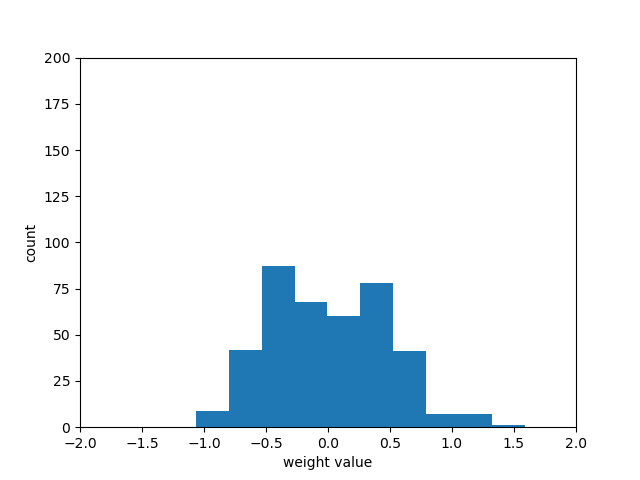
\includegraphics[width=165px]{images/weight_histogram_0.png}
		\centering
		\caption{\small No regularization}
	\end{subfigure}
	\begin{subfigure}{.5\linewidth}
		\centering
		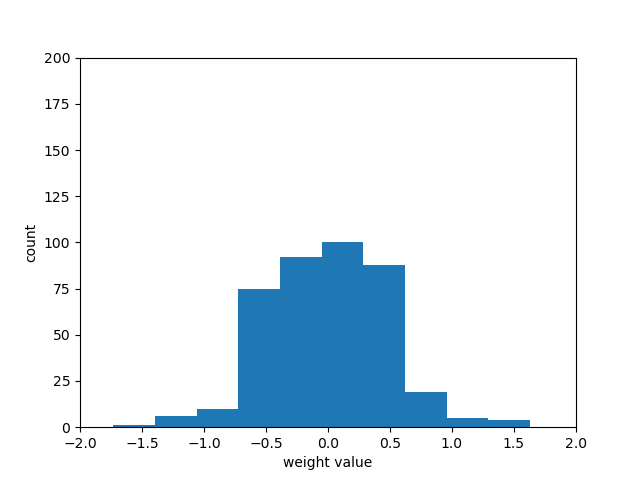
\includegraphics[width=165px]{images/weight_histogram_0_1.png}
		\caption{\small L2 regularization $\lambda = 0.1$}
	\end{subfigure}
	\caption{Weight distributions}
	\label{fig:weight_histogram}
\end{figure}

Finally, figure \ref{fig:learning_process} shows an example of the learning process and the outputs of our selected network with 8 nodes in the hidden layer, a learning rate of 0.1 and an L2 weight decay with $\lambda = 0.1$. The MSE on the test set of such a network can be seen in table \ref{tab:learning_outcomes}. The best of the 10 tested networks had an MSE of 0.00621 which demonstrates its good generalisation capabilities.

\begin{figure}[h!]
	\begin{subfigure}{.5\linewidth}
		
\includegraphics[width=165px]{images/learning_mse.png}
		\centering
		\caption{\small Learning process}
	\end{subfigure}
	\begin{subfigure}{.5\linewidth}
		\centering
		\includegraphics[width=165px]{images/predictions.png}
		\caption{\small Predictions after training}
	\end{subfigure}
	\caption{Weight distributions}
	\label{fig:learning_process}
\end{figure}

\subsection{Comparison of two- and three-layer perceptron for noisy time series prediction}

\section{Final remarks \normalsize{\textit{(max 0.5 page)}}}
% \textit{Please share your final reflections on the lab, its content and your own learning. Which parts of the lab assignment did you find confusing or not necessarily helping in understanding important concepts and which parts you have found interesting and relevant to your learning experience? \\
% Here you can also formulate your opinion, interpretation or speculation about some of the simulation outcomes. Please add any follow-up questions that you might have regarding the lab tasks and the results you have produced.}

\end{document}
